\documentclass[10pt,aspectratio=169]{beamer}
\usepackage{bma02}

\title[Sustitución trigonométrica e hiperbólicas]{Sustitución trigonométrica}
\subtitle{Primitivas de funciones hiperbólicas\\[2pt]\small Semana 6 -- Sesión 1}

\begin{document}

\begin{frame}
  \titlepage
\end{frame}

\begin{frame}{Objetivos de la sesión}
  \begin{enumerate}
    \item Integrar expresiones con $\sqrt{a^2-x^2}$, $\sqrt{a^2+x^2}$, $\sqrt{x^2-a^2}$ mediante \resaltar{sustitución trigonométrica}.
    \item Usar el triángulo de referencia para regresar a la variable original.
    \item Conocer las \resaltar{funciones hiperbólicas}, sus identidades, derivadas e integrales.
    \item Usar las funciones hiperbólicas inversas y la \resaltar{sustitución hiperbólica}.
  \end{enumerate}
  \vspace{1mm}
  {\small\textbf{Competencia 3 del sílabo:} Desarrolla el pensamiento deductivo, inductivo, crítico y creativo mediante cambios de variable en los métodos de integración.}
  \begin{block}{Plan (2 horas; incluye verificación previa de 5 min)}
    \begin{tabular}{ll}
      0:00 -- 0:55 & Sustitución trigonométrica: tres casos, ejemplos, completar cuadrados\\
      0:55 -- 1:15 & Funciones hiperbólicas: definición, gráficas, identidades\\
      1:15 -- 1:40 & Derivadas, primitivas, inversas, sustitución hiperbólica\\
      1:40 -- 2:00 & Actividad colaborativa, resumen y cierre metacognitivo
    \end{tabular}
  \end{block}
\end{frame}

\begin{frame}{Aula invertida: preparación y verificación}
  \small
  \begin{previa}[antes de la sesión]
    \begin{enumerate}
      \item Lea la sustitución trigonométrica (tres casos) y las funciones hiperbólicas.
      \item Identifique la sustitución para $\sqrt{4-x^2}$, $\sqrt{x^2+4}$ y $\sqrt{x^2-4}$.
      \item Pregunta guía: ¿qué identidad trigonométrica elimina el radical en cada caso?
    \end{enumerate}
  \end{previa}
  \begin{block}{Verificación al inicio (5 min, en pares)}
    \begin{enumerate}
      \item ¿Qué sustitución elimina $\sqrt{9-x^2}$?
      \item Calcule $\cosh^2x-\senh^2x$.
    \end{enumerate}
    Los pares discuten y votan; el docente aclara solo lo que genera dudas y ajusta el ritmo de la sesión.
  \end{block}
\end{frame}

\section{Sustitución trigonométrica}

\begin{frame}{Idea: eliminar la raíz con una identidad pitagórica}
  \renewcommand{\arraystretch}{1.6}
  \begin{center}
  \begin{tabular}{c|c|c|c}
    \textbf{Expresión} & \textbf{Sustitución} & \textbf{Identidad} & \textbf{Rango de $\theta$}\\ \hline
    $\sqrt{a^2-x^2}$ & $x=a\sen\theta$ & $1-\sen^2\theta=\cos^2\theta$ & $-\frac\pi2\le\theta\le\frac\pi2$\\
    $\sqrt{a^2+x^2}$ & $x=a\tan\theta$ & $1+\tan^2\theta=\sec^2\theta$ & $-\frac\pi2<\theta<\frac\pi2$\\
    $\sqrt{x^2-a^2}$ & $x=a\sec\theta$ & $\sec^2\theta-1=\tan^2\theta$ & $0\le\theta<\frac\pi2$ ó $\pi\le\theta<\frac{3\pi}2$
  \end{tabular}
  \end{center}
  \begin{center}
    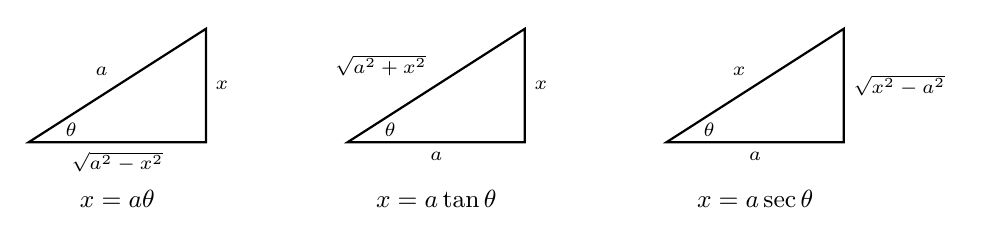
\begin{tikzpicture}[scale=0.9]
      \draw[thick] (0,0) -- (2.5,0) -- (2.5,1.6) -- cycle;
      \node at (0.6,0.18) {\scriptsize $\theta$};
      \node[above left] at (1.25,0.8) {\scriptsize $a$};
      \node[right] at (2.5,0.8) {\scriptsize $x$};
      \node[below] at (1.25,0) {\scriptsize $\sqrt{a^2-x^2}$};
      \node at (1.25,-0.8) {\small $x=a\sen\theta$};
      \begin{scope}[xshift=4.5cm]
        \draw[thick] (0,0) -- (2.5,0) -- (2.5,1.6) -- cycle;
        \node at (0.6,0.18) {\scriptsize $\theta$};
        \node[above left] at (1.25,0.8) {\scriptsize $\sqrt{a^2+x^2}$};
        \node[right] at (2.5,0.8) {\scriptsize $x$};
        \node[below] at (1.25,0) {\scriptsize $a$};
        \node at (1.25,-0.8) {\small $x=a\tan\theta$};
      \end{scope}
      \begin{scope}[xshift=9cm]
        \draw[thick] (0,0) -- (2.5,0) -- (2.5,1.6) -- cycle;
        \node at (0.6,0.18) {\scriptsize $\theta$};
        \node[above left] at (1.25,0.8) {\scriptsize $x$};
        \node[right] at (2.5,0.8) {\scriptsize $\sqrt{x^2-a^2}$};
        \node[below] at (1.25,0) {\scriptsize $a$};
        \node at (1.25,-0.8) {\small $x=a\sec\theta$};
      \end{scope}
    \end{tikzpicture}
  \end{center}
  \small Los triángulos de referencia permiten expresar $\sen\theta,\cos\theta,\tan\theta,\dots$ en términos de $x$.
\end{frame}

\begin{frame}{Caso 1: $\sqrt{a^2-x^2}$, \ $x=a\sen\theta$}
  \begin{ejemplo}[1]
    $\displaystyle\int\frac{\sqrt{9-x^2}}{x^2}\dx$. \quad $x=3\sen\theta$, $dx=3\cos\theta\dth$, $\sqrt{9-x^2}=3\cos\theta$:
    \[ \int\frac{3\cos\theta}{9\sen^2\theta}\,3\cos\theta\dth=\int\ctg^2\theta\dth=\int(\cosec^2\theta-1)\dth=-\ctg\theta-\theta+C. \]
    Del triángulo: $\ctg\theta=\dfrac{\sqrt{9-x^2}}{x}$, \ $\theta=\arcsen\dfrac x3$:
    \[ \int\frac{\sqrt{9-x^2}}{x^2}\dx=-\frac{\sqrt{9-x^2}}{x}-\arcsen\frac x3+C. \]
  \end{ejemplo}
  \begin{ejemplo}[2: definida, área de la elipse]
    $\displaystyle A=4\int_0^a\frac ba\sqrt{a^2-x^2}\dx\overset{x=a\sen\theta}{=}4ab\int_0^{\pi/2}\cos^2\theta\dth=\pi ab.$
  \end{ejemplo}
\end{frame}

\begin{frame}{Caso 2: $\sqrt{a^2+x^2}$, \ $x=a\tan\theta$}
  \begin{ejemplo}[3]
    $\displaystyle\int\frac{dx}{x^2\sqrt{x^2+4}}$. \quad $x=2\tan\theta$, $dx=2\sec^2\theta\dth$, $\sqrt{x^2+4}=2\sec\theta$:
    \[ \int\frac{2\sec^2\theta}{4\tan^2\theta\cdot2\sec\theta}\dth=\frac14\int\frac{\cos\theta}{\sen^2\theta}\dth=-\frac{1}{4\sen\theta}+C
      =-\frac{\sqrt{x^2+4}}{4x}+C. \]
  \end{ejemplo}
  \begin{ejemplo}[4: una integral muy usada]
    $\displaystyle\int\sqrt{x^2+1}\dx\overset{x=\tan\theta}{=}\int\sec^3\theta\dth=\tfrac12\big(\sec\theta\tan\theta+\ln|\sec\theta+\tan\theta|\big)+C$
    \[ =\frac12\left(x\sqrt{x^2+1}+\ln\big(x+\sqrt{x^2+1}\big)\right)+C. \]
    Aplicación: la longitud de la parábola $y=\frac{x^2}{2}$, $0\le x\le1$, es $\frac12\left(\sqrt2+\ln(1+\sqrt2)\right)\approx1.148$.
  \end{ejemplo}
\end{frame}

\begin{frame}{Caso 3: $\sqrt{x^2-a^2}$, \ $x=a\sec\theta$}
  \begin{ejemplo}[5]
    $\displaystyle\int\frac{dx}{\sqrt{x^2-a^2}}$, $x>a$. \quad $x=a\sec\theta$, $dx=a\sec\theta\tan\theta\dth$, $\sqrt{x^2-a^2}=a\tan\theta$:
    \[ \int\sec\theta\dth=\ln|\sec\theta+\tan\theta|+C_1=\ln\left|\frac xa+\frac{\sqrt{x^2-a^2}}{a}\right|+C_1
       =\ln\left|x+\sqrt{x^2-a^2}\right|+C. \]
  \end{ejemplo}
  \begin{ejemplo}[6]
    $\displaystyle\int_{2}^{4}\frac{\sqrt{x^2-4}}{x}\dx$. \quad $x=2\sec\theta$, $\theta:0\to\frac\pi3$:
    \[ \int_0^{\pi/3}\frac{2\tan\theta}{2\sec\theta}\,2\sec\theta\tan\theta\dth=2\int_0^{\pi/3}(\sec^2\theta-1)\dth=2\sqrt3-\frac{2\pi}3. \]
  \end{ejemplo}
\end{frame}

\begin{frame}{Completar cuadrados}
  \begin{ejemplo}[7]
    $\displaystyle\int\frac{x}{\sqrt{3-2x-x^2}}\dx$. \quad $3-2x-x^2=4-(x+1)^2$. \ Sea $x+1=2\sen\theta$:
    \[ \int\frac{2\sen\theta-1}{2\cos\theta}\,2\cos\theta\dth=-2\cos\theta-\theta+C
       =-\sqrt{3-2x-x^2}-\arcsen\frac{x+1}{2}+C. \]
  \end{ejemplo}
  \begin{ejemplo}[8: ¡no siempre hace falta!]
    $\displaystyle\int\frac{x}{\sqrt{x^2+4}}\dx=\sqrt{x^2+4}+C$ \ con $u=x^2+4$. \ Primero busque una sustitución simple.
  \end{ejemplo}
  \begin{block}{Recomendaciones}
    \begin{itemize}
      \item Use el rango de $\theta$ indicado para que $\sqrt{\cos^2\theta}=\cos\theta$, etc.
      \item En integrales definidas, cambie los límites y evite regresar a $x$.
      \item Para potencias $(a^2+x^2)^{n/2}$, también sirve la sustitución.
    \end{itemize}
  \end{block}
\end{frame}

\section{Funciones hiperbólicas}

\begin{frame}{Definición y gráficas}
  \begin{columns}
    \begin{column}{0.5\textwidth}
      \begin{definicion}
        \[ \senh x=\frac{e^x-e^{-x}}{2},\qquad \cosh x=\frac{e^x+e^{-x}}{2}, \]
        \[ \tanh x=\frac{\senh x}{\cosh x},\quad \sech x=\frac1{\cosh x},\ \dots \]
      \end{definicion}
      \begin{proposicion}[identidades]
        \begin{itemize}
          \item $\cosh^2x-\senh^2x=1$
          \item $1-\tanh^2x=\sech^2x$
          \item $\senh2x=2\senh x\cosh x$
          \item $\cosh2x=\cosh^2x+\senh^2x$
        \end{itemize}
      \end{proposicion}
    \end{column}
    \begin{column}{0.5\textwidth}
      \centering
      \begin{tikzpicture}
        \begin{axis}[bma, xmin=-2.6, xmax=2.6, ymin=-3.2, ymax=3.6, width=7cm, height=6.5cm, xtick={-2,-1,1,2}, ytick={-1,1}, domain=-2.5:2.5]
          \addplot[curva2, domain=-1.9:1.9] {cosh(x)};
          \addplot[curva, domain=-1.85:1.85] {sinh(x)};
          \addplot[uniVerde, very thick] {tanh(x)};
          \addplot[gray, dashed, domain=-2.5:2] {exp(x)/2};
          \node[uniGranate] at (axis cs:1.3,3.2) {\scriptsize $\cosh x$};
          \node[uniAzul] at (axis cs:2.05,2.4) {\scriptsize $\senh x$};
          \node[uniVerde] at (axis cs:2.2,0.65) {\scriptsize $\tanh x$};
          \node[gray] at (axis cs:-1.6,0.6) {\scriptsize $\frac{e^x}2$};
        \end{axis}
      \end{tikzpicture}
    \end{column}
  \end{columns}
\end{frame}

\begin{frame}{¿Por qué ``hiperbólicas''?}
  \begin{columns}
    \begin{column}{0.5\textwidth}
      \begin{itemize}
        \item $(\cos t,\sen t)$ recorre la circunferencia $x^2+y^2=1$.
        \item $(\cosh t,\senh t)$ recorre la rama derecha de la hipérbola $x^2-y^2=1$.
      \end{itemize}
      \begin{observacion}
        En ambos casos el área del sector sombreado es $\dfrac t2$ (compruébelo con la fórmula de la sesión anterior).
        El parámetro $t$ juega el papel de ``ángulo hiperbólico''.
      \end{observacion}
      \small En relatividad especial, la \emph{rapidez} (rapidity) es un ángulo hiperbólico y las transformaciones de Lorentz son
      ``rotaciones hiperbólicas''.
    \end{column}
    \begin{column}{0.5\textwidth}
      \centering
      \begin{tikzpicture}
        \begin{axis}[bma, xmin=-1.3, xmax=3, ymin=-2, ymax=2, axis equal image, width=7cm, height=6.3cm, xtick={1}, ytick={1}]
          \addplot[fill=uniGranate!25, draw=none, domain=0:1, samples=50] ({cosh(x)},{sinh(x)}) -- (axis cs:0,0) -- cycle;
          \addplot[fill=uniAzul!30, draw=none, domain=0:57.3, samples=50] ({cos(x)},{sin(x)}) -- (axis cs:0,0) -- cycle;
          \addplot[curva, domain=0:360, samples=100] ({cos(x)},{sin(x)});
          \addplot[curva2, domain=-1.4:1.4, samples=100] ({cosh(x)},{sinh(x)});
          \draw[uniGranate] (axis cs:0,0) -- (axis cs:1.543,1.175);
          \node[uniGranate, right] at (axis cs:1.55,1.17) {\scriptsize $(\cosh t,\senh t)$};
          \node[uniAzul, above] at (axis cs:0.4,0.9) {\scriptsize $(\cos t,\sen t)$};
        \end{axis}
      \end{tikzpicture}
    \end{column}
  \end{columns}
\end{frame}

\begin{frame}{Derivadas y primitivas}
  \begin{columns}[t]
    \begin{column}{0.5\textwidth}
      \begin{block}{Derivadas}
        \begin{align*}
          (\senh x)'&=\cosh x & (\cosh x)'&=\senh x\\
          (\tanh x)'&=\sech^2x & (\coth x)'&=-\csch^2x\\
          (\sech x)'&=-\sech x\tanh x
        \end{align*}
        \vspace{-4mm}
      \end{block}
    \end{column}
    \begin{column}{0.5\textwidth}
      \begin{block}{Primitivas}
        \begin{align*}
          \textstyle\int\senh x\dx&=\cosh x+C\\
          \textstyle\int\cosh x\dx&=\senh x+C\\
          \textstyle\int\tanh x\dx&=\ln(\cosh x)+C\\
          \textstyle\int\sech x\dx&=\arctan(\senh x)+C
        \end{align*}
        \vspace{-4mm}
      \end{block}
    \end{column}
  \end{columns}
  \begin{ejemplo}
    $\displaystyle\int\senh^2x\dx=\int\frac{\cosh2x-1}{2}\dx=\frac{\senh2x}{4}-\frac x2+C$. \quad
    $\displaystyle\int\senh^3x\cosh x\dx=\frac{\senh^4x}{4}+C$.
  \end{ejemplo}
  \small Las fórmulas son como las trigonométricas, salvo cambios de signo (regla de Osborn).
\end{frame}

\begin{frame}{Funciones hiperbólicas inversas}
  \begin{proposicion}[expresiones logarítmicas]
    \begin{align*}
      \arcsenh x&=\ln\big(x+\sqrt{x^2+1}\big),\ x\in\R; &
      \arccosh x&=\ln\big(x+\sqrt{x^2-1}\big),\ x\ge1;\\
      \arctanh x&=\frac12\ln\frac{1+x}{1-x},\ |x|<1.
    \end{align*}
  \end{proposicion}
  \textbf{Prueba} ($\arcsenh$). $y=\arcsenh x\iff x=\frac{e^y-e^{-y}}{2}\iff e^{2y}-2xe^y-1=0\iff e^y=x+\sqrt{x^2+1}$ (raíz positiva).
  \begin{teorema}[primitivas que producen hiperbólicas inversas]
    \[ \int\frac{dx}{\sqrt{x^2+a^2}}=\arcsenh\frac xa+C,\quad \int\frac{dx}{\sqrt{x^2-a^2}}=\arccosh\frac xa+C,\quad
       \int\frac{dx}{a^2-x^2}=\frac1a\arctanh\frac xa+C. \]
  \end{teorema}
  \small Compare con el Ejemplo 5: $\arccosh\frac xa=\ln\big(x+\sqrt{x^2-a^2}\big)-\ln a$. ¡Solo difieren en una constante!
\end{frame}

\begin{frame}{Sustitución hiperbólica}
  Alternativa a la sustitución trigonométrica: \ $x=a\senh t$ para $\sqrt{a^2+x^2}$ \ y \ $x=a\cosh t$ para $\sqrt{x^2-a^2}$.
  \begin{ejemplo}[9]
    $\displaystyle\int\sqrt{x^2+a^2}\dx$, \ $x=a\senh t$, $dx=a\cosh t\dt$, $\sqrt{x^2+a^2}=a\cosh t$:
    \[ a^2\int\cosh^2t\dt=\frac{a^2}2\int(1+\cosh2t)\dt=\frac{a^2}2\left(t+\senh t\cosh t\right)+C \]
    \[ =\frac12x\sqrt{x^2+a^2}+\frac{a^2}2\arcsenh\frac xa+C. \]
  \end{ejemplo}
  \begin{ejemplo}[10: física, caída con resistencia del aire]
    Con $m\,v'=mg-kv^2$, separando variables: $\displaystyle\int\frac{dv}{g-\frac km v^2}=t$ \ $\Rightarrow$ \
    $v(t)=\sqrt{\tfrac{mg}{k}}\tanh\!\left(\sqrt{\tfrac{gk}{m}}\,t\right)$. \ La velocidad terminal es $\sqrt{mg/k}$.
  \end{ejemplo}
\end{frame}

\begin{frame}{Actividad colaborativa: Expertos por caso}
  \small
  \begin{activa}[Enseñanza entre pares (rompecabezas)]
    Tres grupos de expertos resuelven $\int\sqrt{4-x^2}\,dx$, $\int\frac{dx}{\sqrt{x^2+4}}$ y $\int\frac{\sqrt{x^2-9}}{x}\,dx$. Regresan a grupos mixtos, enseñan su caso y resuelven juntos el área de la elipse $\frac{x^2}{9}+\frac{y^2}{4}=1$.
  \end{activa}
  \begin{itemize}
    \item \textbf{Organización:} equipos de 3 a 4 con roles rotativos (coordinador, redactor, verificador, portavoz); 12--15 minutos.
    \item \textbf{Producto:} Tres resoluciones comentadas y el área de la elipse.
    \item \textbf{Retroalimentación:} el docente recorre los equipos, hace preguntas y no da la solución hasta la puesta en común.
  \end{itemize}
\end{frame}

\section{Ejercicios}

\begin{frame}{Ejercicios propuestos}
  \begin{ejercicio}
    \begin{multicols}{2}
    \begin{enumerate}
      \item $\displaystyle\int\frac{x^2}{\sqrt{4-x^2}}\dx$
      \item $\displaystyle\int\frac{dx}{(x^2+9)^{3/2}}$
      \item $\displaystyle\int\frac{\sqrt{x^2-1}}{x^4}\dx$
      \item $\displaystyle\int x^3\sqrt{1-x^2}\dx$ \ \small(¿hace falta?)
      \item $\displaystyle\int\frac{dx}{\sqrt{x^2+6x+13}}$
      \item $\displaystyle\int_0^{1}\frac{x^3}{\sqrt{x^2+1}}\dx$
      \item $\displaystyle\int\frac{e^x}{\sqrt{e^{2x}-1}}\dx$
      \item $\displaystyle\int\cosh^2(3x)\dx$
      \item $\displaystyle\int\frac{\senh x}{1+\cosh x}\dx$
      \item $\displaystyle\int\frac{dx}{\sqrt{4x^2-1}}$ (dos formas)
    \end{enumerate}
    \end{multicols}
  \end{ejercicio}
  \begin{ejercicio}[: aplicaciones]
    \begin{enumerate}
      \setcounter{enumi}{10}
      \item Halle la longitud de la espiral $r=\theta$, $0\le\theta\le2\pi$ (planteada la sesión anterior).
      \item Pruebe que el área del sector hiperbólico entre $(0,0)$, $(1,0)$ y $(\cosh t,\senh t)$ es $t/2$.
    \end{enumerate}
  \end{ejercicio}
\end{frame}

\begin{frame}{Metacognición y uso responsable de la IA}
  \small
  \begin{columns}[t]
    \begin{column}{0.5\textwidth}
      \begin{metacog}[cierre, 3 min]
        \begin{enumerate}
          \metacomun
          \item ¿Pude explicar el cambio de variable a un compañero? ¿Qué parte me costó más?
        \end{enumerate}
      \end{metacog}
    \end{column}
    \begin{column}{0.5\textwidth}
      \begin{iabox}
        Pida a una IA $\int\frac{dx}{\sqrt{x^2+4}}$ por sustitución trigonométrica y por hiperbólica. Compare ambas respuestas y explique por qué son equivalentes.\\[2pt]
        \textit{Regla:} primero intente usted; luego use la herramienta para contrastar, nunca para sustituir su razonamiento. Anote el cambio en su bitácora.
      \end{iabox}
    \end{column}
  \end{columns}
\end{frame}

\begin{frame}{Resumen}
  \begin{itemize}
    \item $\sqrt{a^2-x^2}$: $x=a\sen\theta$; \ $\sqrt{a^2+x^2}$: $x=a\tan\theta$; \ $\sqrt{x^2-a^2}$: $x=a\sec\theta$.
    \item Regresar a $x$ con el triángulo de referencia; completar cuadrados si hay término lineal.
    \item $\cosh^2-\senh^2=1$; \ $(\senh)'=\cosh$, $(\cosh)'=\senh$.
    \item $\arcsenh x=\ln(x+\sqrt{x^2+1})$, etc.; \ $\int\frac{dx}{\sqrt{x^2\pm a^2}}=\ln|x+\sqrt{x^2\pm a^2}|+C$.
  \end{itemize}
  \vspace{3mm}
  \textbf{Próxima sesión:} integración de funciones racionales por fracciones parciales.
\end{frame}


\begin{frame}{Evaluación y trabajo posterior}
  \small
  \begin{evalbox}[Práctica del miércoles de la semana 6: Calificada 2]
    \textbf{Cobertura:} semanas 3 y 4. \textbf{Naturaleza:} práctica calificada individual escrita.
  \end{evalbox}
  \begin{itemize}
    \item \criterios
    \item \declaracionia
    \item \textbf{Portafolio:} guarde el producto de la actividad, la bitácora de metacognición y los ejercicios propuestos de esta sesión; son evidencia de progreso y base de la retroalimentación.
  \end{itemize}
\end{frame}

\end{document}
